\message{ !name(Algorithms.tex)}\documentclass{article}
\usepackage{times}
\usepackage{xeCJK}
\usepackage{graphicx}
\graphicspath{{./}}

\begin{document}

\message{ !name(Algorithms.tex) !offset(-3) }

\title{ Note for reading algorithms }
\author{Guozhen}
\date{\today}
\maketitle

\section{Formula}
\label{sec:Formula}

\begin{itemize}
\item 调和级数求和:$H_n=1+1/2+1/3+1/4 \cdots +1/N \sim lnN$
\item 等差数列求和:$1+2+3+4+ \cdots +N \sim N^2/2$
\item 等比数列求和:$1+2+4+8+ \cdots +N \sim 2N$,其中 $N=2^n$
\item 斯特灵公式:$lgN!=lg1+lg2+lg3+lg4+ \cdots +lgN \sim NlgN$
\item 二项式系数:$\binom{N}{k} \sim N^k/k!$, 其中k为小常数
\item 指数函数:$(1-1/x)^x \sim 1/e$
\end{itemize}

\begin{figure}
  \centering
  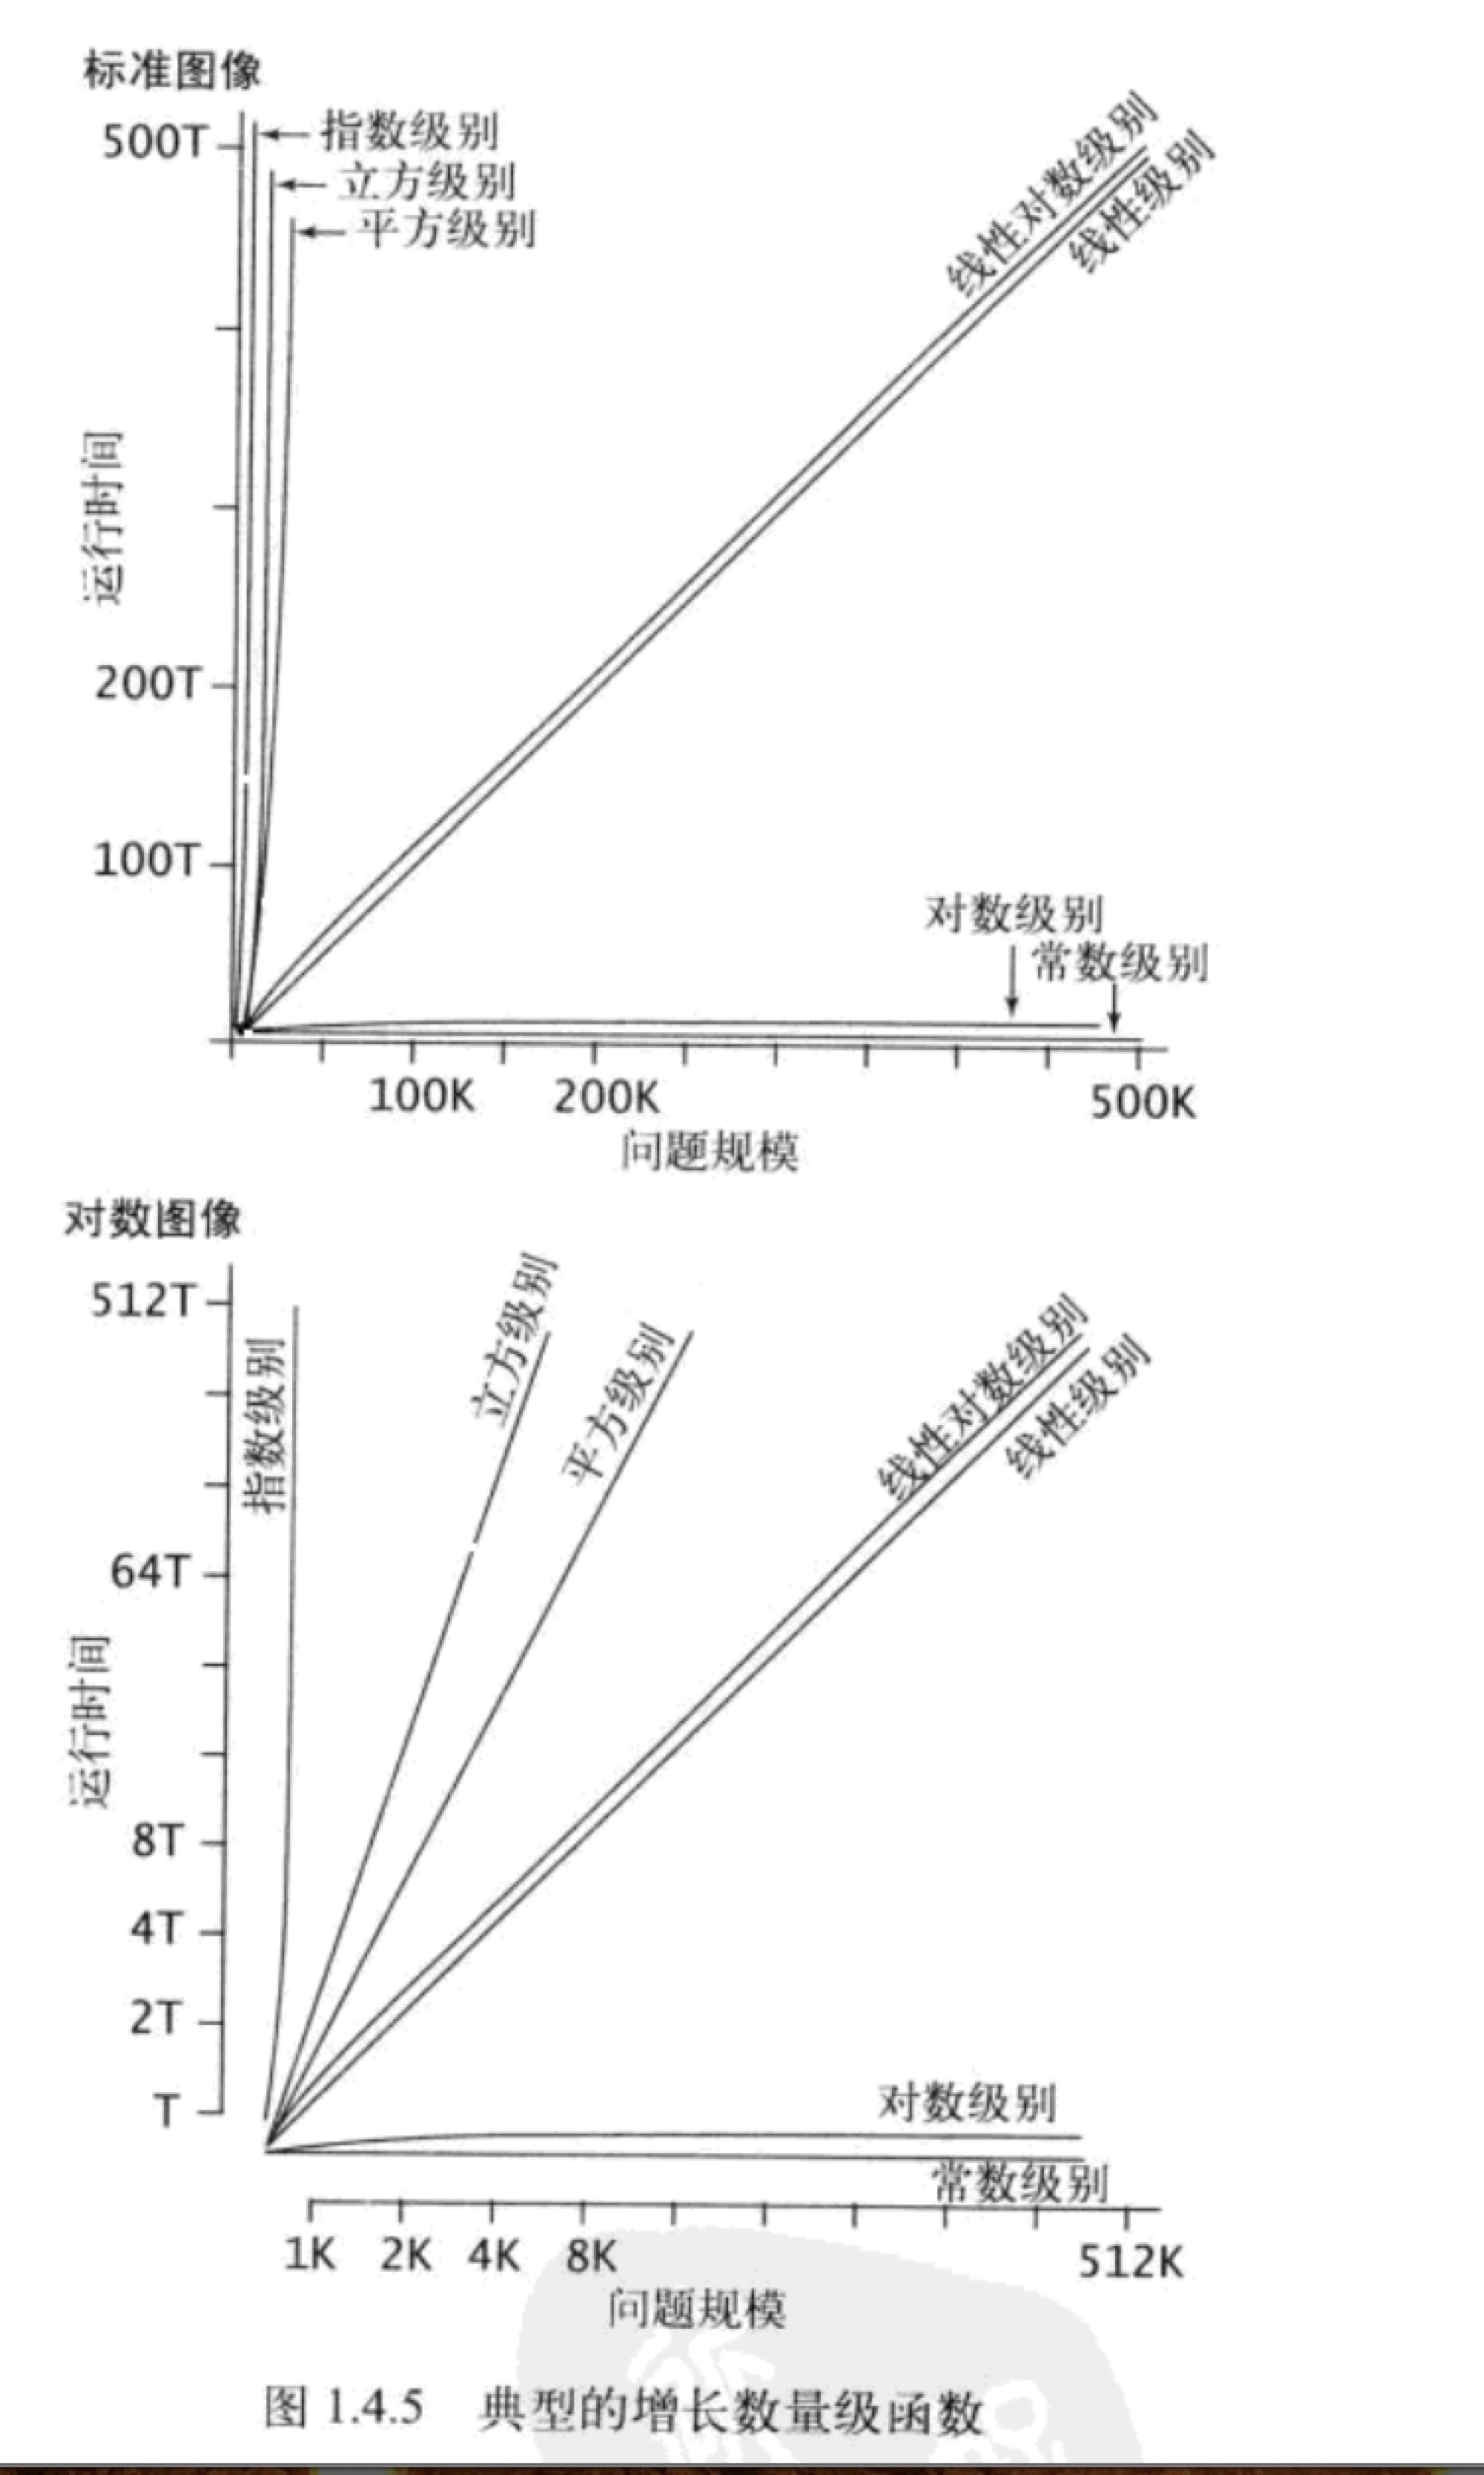
\includegraphics[width=8cm]{chart}
\end{figure}

\end{document}

\message{ !name(Algorithms.tex) !offset(-35) }
